\documentclass[conference]{IEEEtran}
\usepackage{amsmath,amssymb,graphicx,booktabs,url}
\usepackage[hidelinks]{hyperref}
\graphicspath{{figures/}{figures/component_study/}{figures/visio_revision/}}
\makeatletter
\newenvironment{inlinefigure}{\par\smallskip\noindent\begin{minipage}{\columnwidth}\centering\def\@captype{figure}}{\end{minipage}\par\smallskip}
\newenvironment{inlinetable}{\par\smallskip\noindent\begin{minipage}{\columnwidth}\centering\def\@captype{table}}{\end{minipage}\par\smallskip}
\makeatother
\title{Component Selection for HAUV Aerial--Underwater Target Tracking with Deep Reinforcement Learning}
\author{\IEEEauthorblockN{Jiaqing Wang\textsuperscript{1,*}, Ruixuan Hu\textsuperscript{1} and Zheng Zeng\textsuperscript{1}}
\IEEEauthorblockA{\textsuperscript{1}School of Oceanography, Shanghai Jiao Tong University, Shanghai, China\\
\textsuperscript{*}Corresponding author: Jiaqing Wang\quad\textit{UT27 Student Poster Competition}}}
\begin{document}
\raggedbottom
\maketitle
\begin{abstract}
Tracking a descending water target requires a hybrid aerial underwater vehicle (HAUV) to coordinate visual estimation and propulsion across the air--water interface. We present a common framework combining stereo detection, Kalman estimation and deep reinforcement learning. We compare two visual front ends and three state representations through 1,200 software-in-the-loop tracking trials. The vehicle pursues the target in air and selects its water entry through feedback control. With a shared YOLO26n detector, action contrast achieves the highest observed complete-mission counts, with 63/100 straight-pursuit and 72/100 maneuvering successes. Reliability interventions reveal different representation sensitivities. Lake recordings illustrate physical approach and water entry. Control weights and scenario videos are released on the project website.
\end{abstract}
\begin{IEEEkeywords}
HAUV, aerial--underwater tracking, visual estimation, deep reinforcement learning
\end{IEEEkeywords}

\section{Introduction}
Hybrid aerial underwater vehicles combine aerial mobility with underwater operation~\cite{nezha}. Following a target that descends below the surface requires both modes within one mission. Refraction, changing visibility and propulsion authority make isolated detector accuracy insufficient for selecting a tracking system. We connect perception and control through a shared estimated state, then compare visual front ends and policy representations under matched training budgets. Figure~\ref{fig:mission} illustrates the pursuit concept. The study examines which component combinations maintain acquisition, aerial pursuit and sustained submerged following.

\begin{inlinefigure}
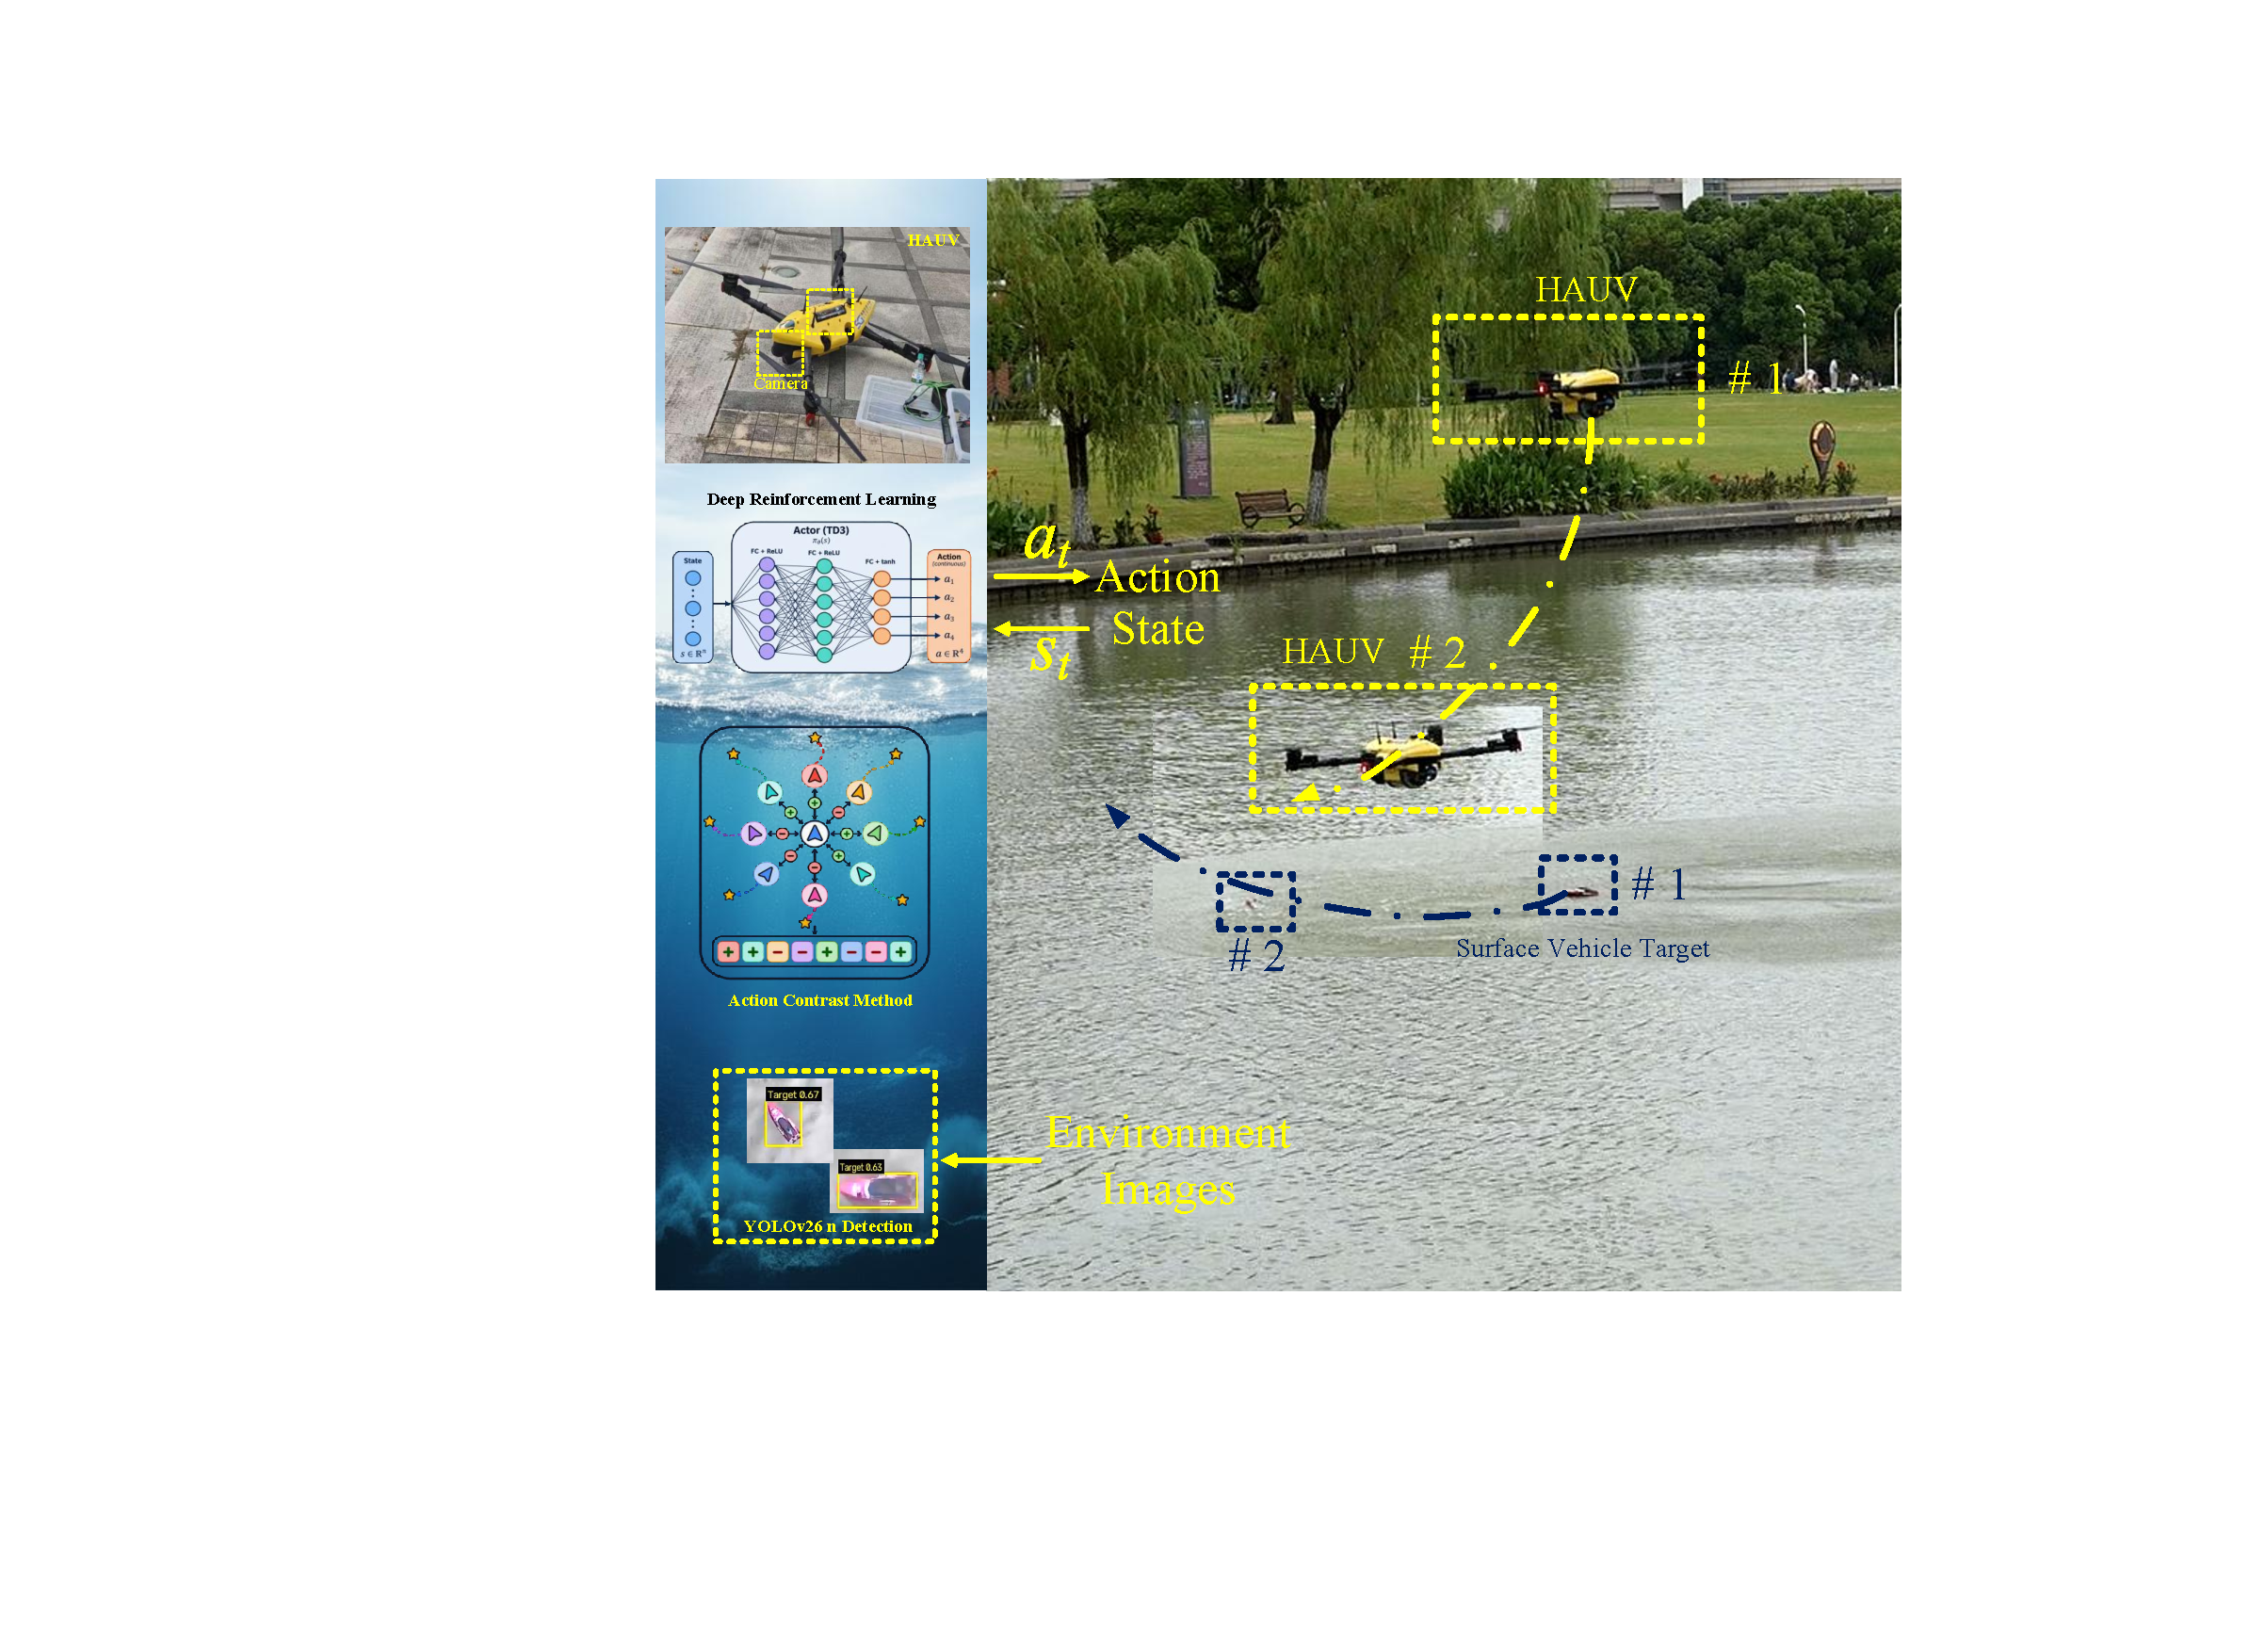
\includegraphics[width=.83\columnwidth]{fig_front.pdf}
\caption{HAUV pursuit concept, physical platform and perception--control components.}
\label{fig:mission}
\end{inlinefigure}

\newpage
\section{Problem Formulation}
The HAUV acquires a near-surface target, pursues it in air and enters water to continue non-contact following. With vehicle position $p_H$, estimated target position $\hat p_T$ and yaw rotation $R_\psi$, the relative estimate and desired offset are
\begin{equation}
\hat r=R_\psi^\top(\hat p_T-p_H),\qquad d=(1.2,0,-1)^\top\;\mathrm{m}.
\end{equation}
True target state supplies rewards and scoring, never actor inputs. Coordinates retain estimated geometry. Directional confidence encoding (DCE) weights bearing by reliability. Action contrast (AC) compares predicted action costs. Field denotes physical lake observations or lake-derived appearance, not a curved trajectory.

\section{Method}
YOLO26n~\cite{yolo} or an ORB template detector~\cite{orb} feeds shared stereo processing and a Kalman filter. Encoders combine estimates, vehicle measurements, reliability and previous commands into 36 coordinate, 45 DCE or 41 AC inputs. AC compares eight command perturbations with the previous command using one-second predictions. Two-layer actors request velocity and yaw rate from a shared propulsion controller. Three seeds share behavior-cloning initialization, Twin Delayed Deep Deterministic Policy Gradient (TD3)~\cite{td3} training budgets and validation-based checkpoint selection. Three selected policies retain initialization. Figure~\ref{fig:components} reserves the component-view layout.

\begin{inlinefigure}
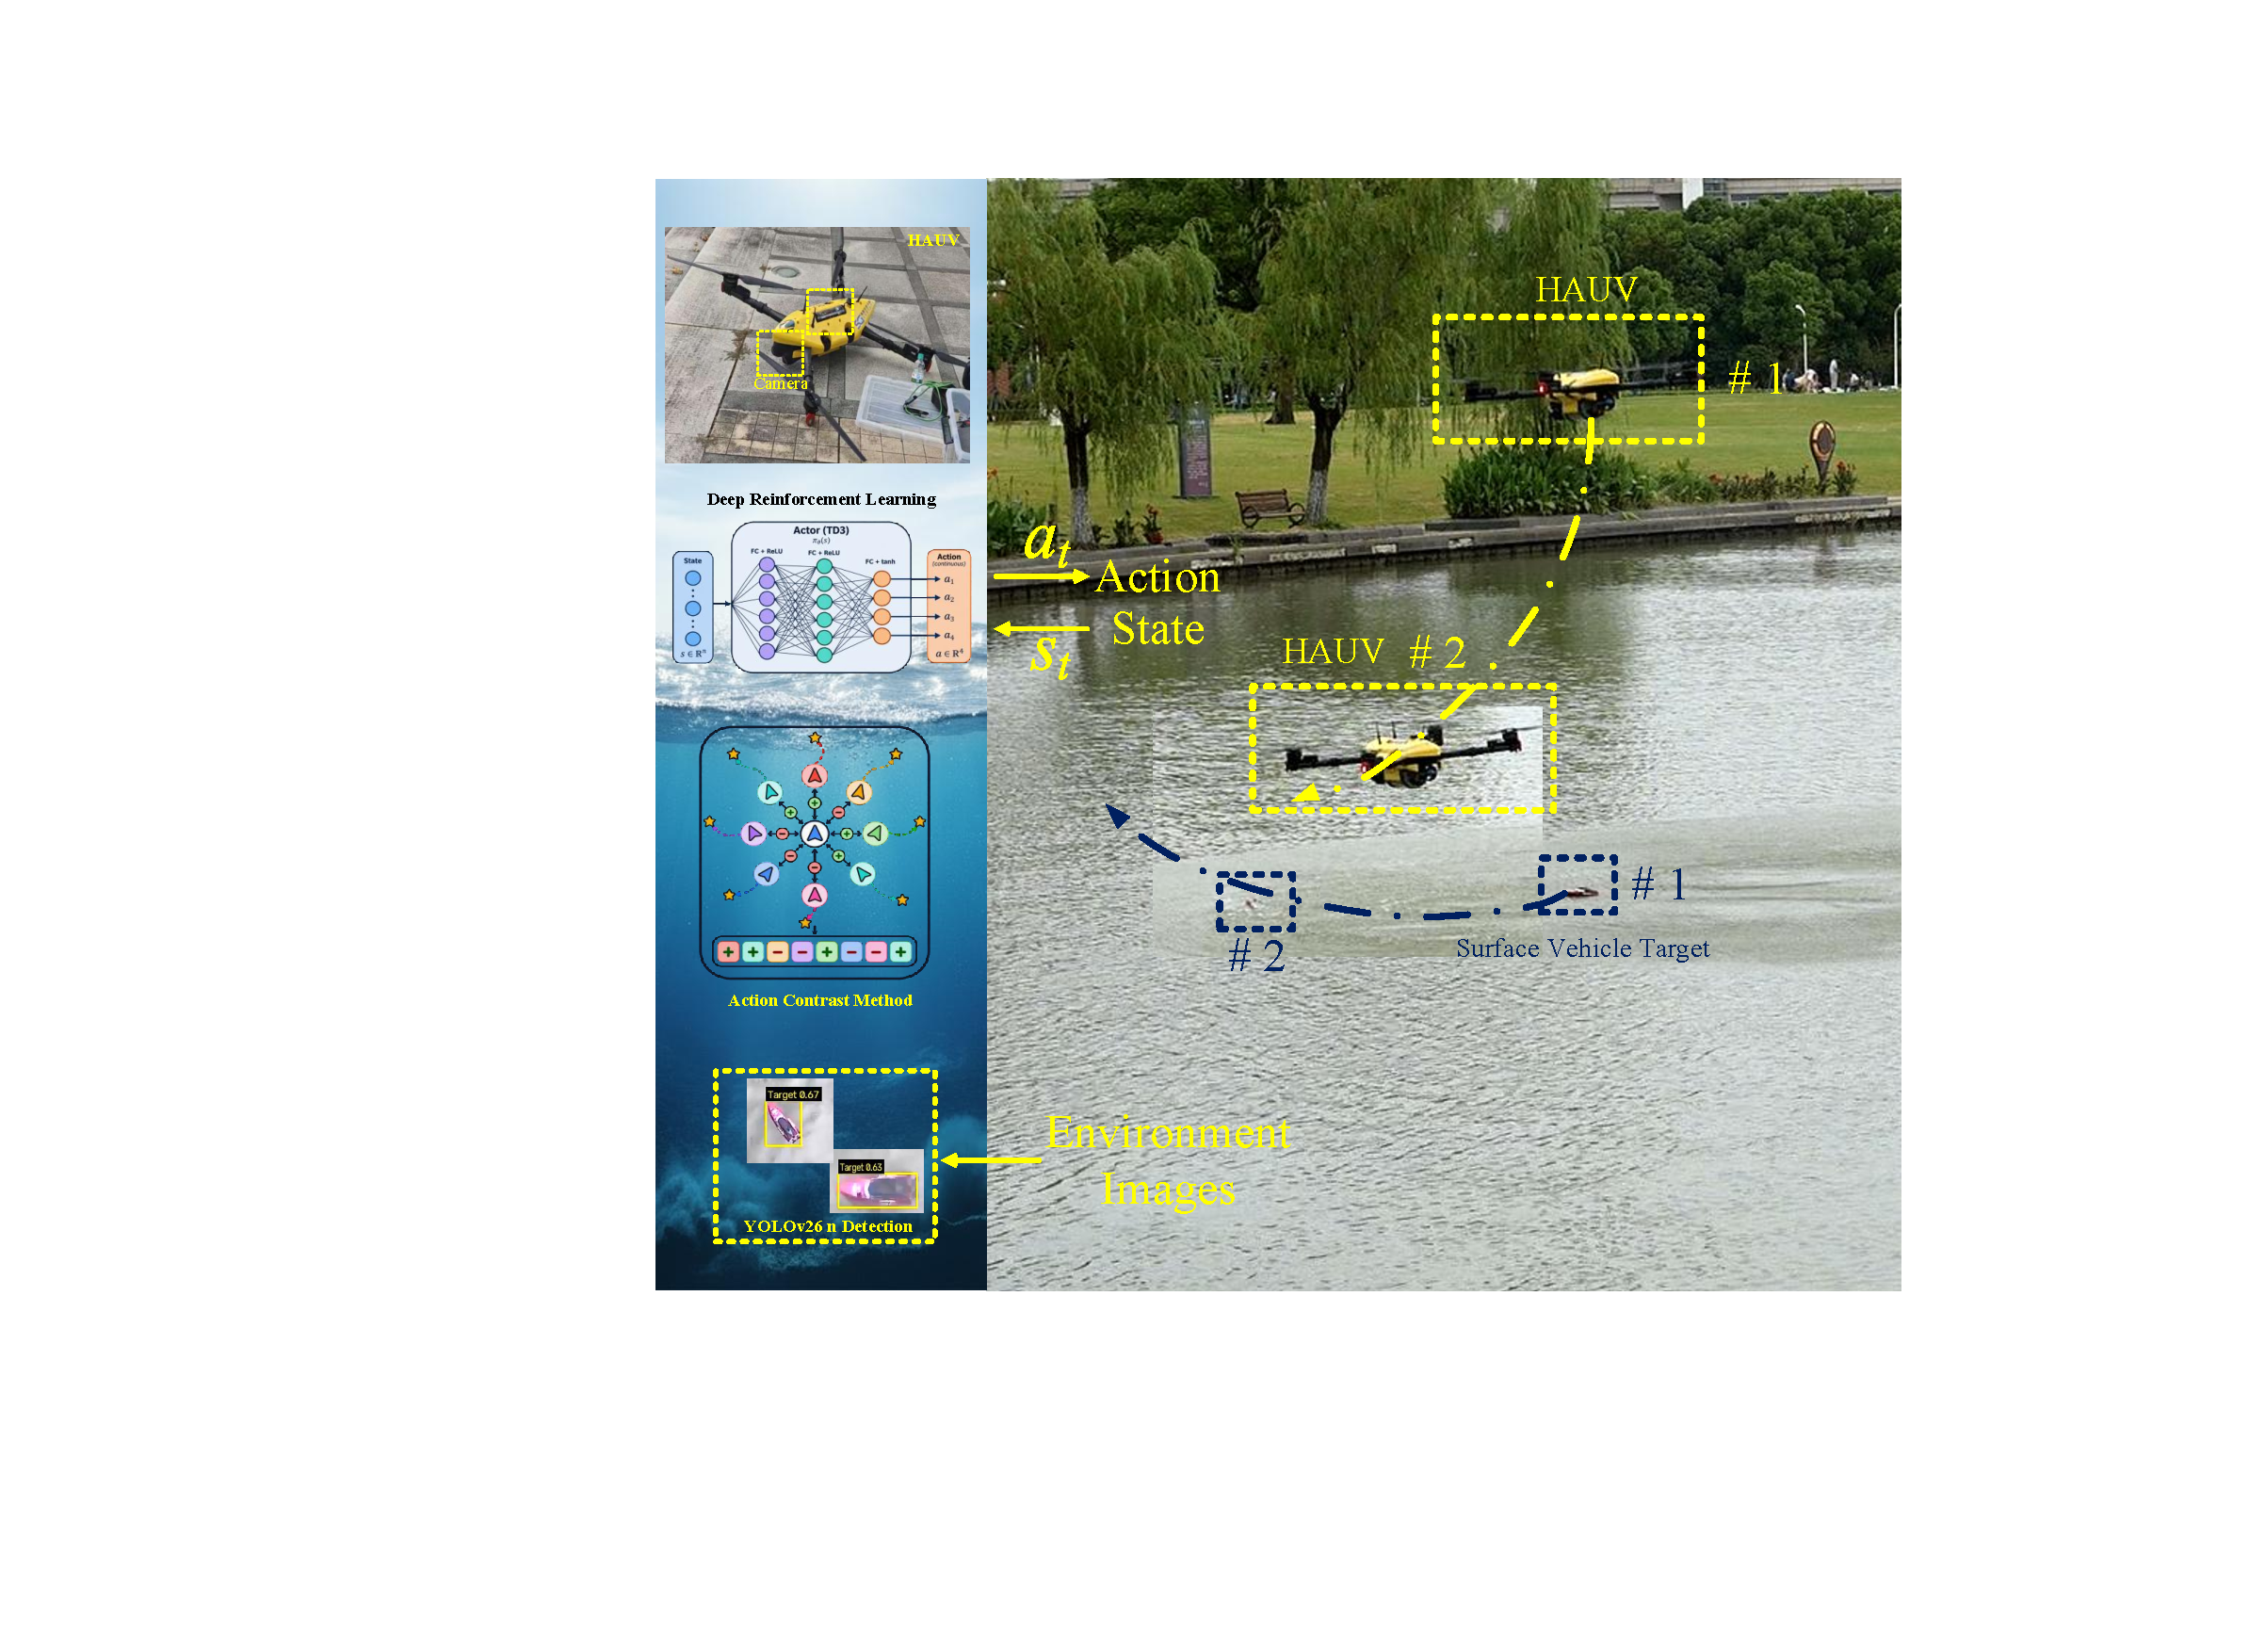
\includegraphics[width=.70\columnwidth]{fig_front.pdf}
\caption{Component-view placeholder, intentionally retaining the image used in Fig.~\ref{fig:mission}.}
\label{fig:components}
\end{inlinefigure}

\clearpage
\section{Experiment}
Isaac Sim renders stereo images with reflection, refraction and scattering; an external reduced six-degree-of-freedom plant uses published Nezha-Mini parameters~\cite{nezha}. Control and cameras run at 10 and 5 Hz. Each detector--representation pair has 100 trials per scenario, split equally between native and lake-appearance rendering. Policies remain frozen. Straight pursuit and maneuvering both require a descending target to be followed underwater. The latter includes a 30--32 s observation gap. Success requires acquisition, aerial closure, sustained underwater following and a valid final approach within a complete 60 s mission.

\begin{inlinefigure}
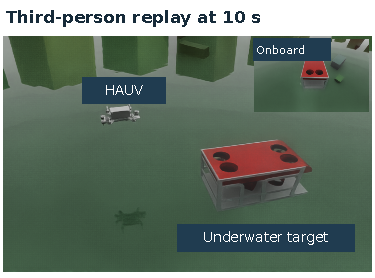
\includegraphics[width=.33\columnwidth]{fig_S1.pdf}\hfill
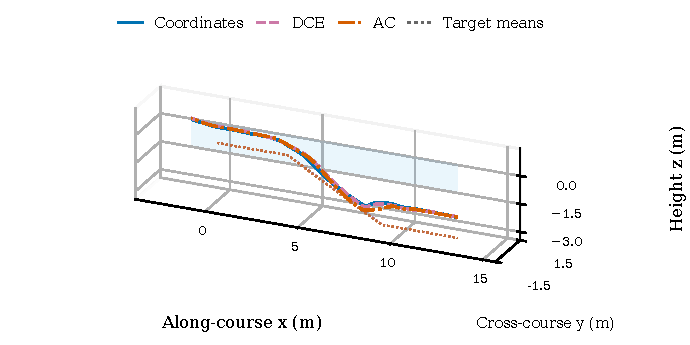
\includegraphics[width=.63\columnwidth]{straight_b_mean3d.pdf}\\[-1mm]
{\footnotesize (a) Camera views\hspace{12mm}(b) Mean trajectories}\\[1mm]
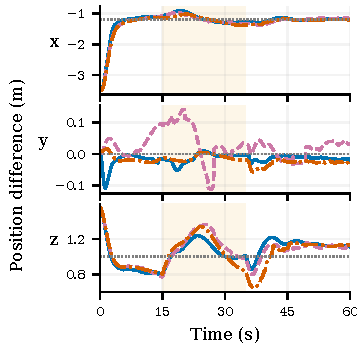
\includegraphics[width=.32\columnwidth]{straight_c_relative.pdf}\hfill
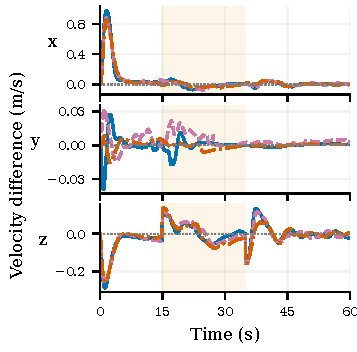
\includegraphics[width=.32\columnwidth]{straight_d_velocity.pdf}\hfill
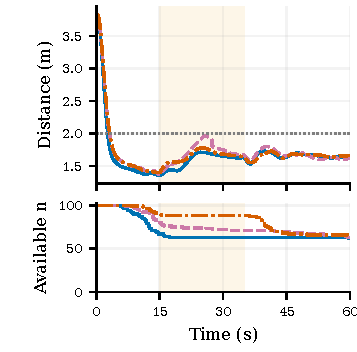
\includegraphics[width=.32\columnwidth]{straight_e_distance_count.pdf}\\[-1mm]
{\footnotesize (c) Relative position\hfill(d) Velocity\hfill(e) Range/count}
\caption{Straight pursuit. All panels retain the shared-YOLO comparison. Means use available executed samples; (e) exposes early termination. Tan shading marks target descent.}
\label{fig:straight}
\end{inlinefigure}

\begin{inlinefigure}
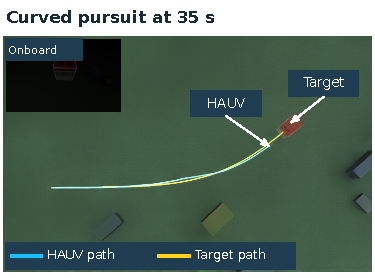
\includegraphics[width=.33\columnwidth]{fig_S2_traj.pdf}\hfill
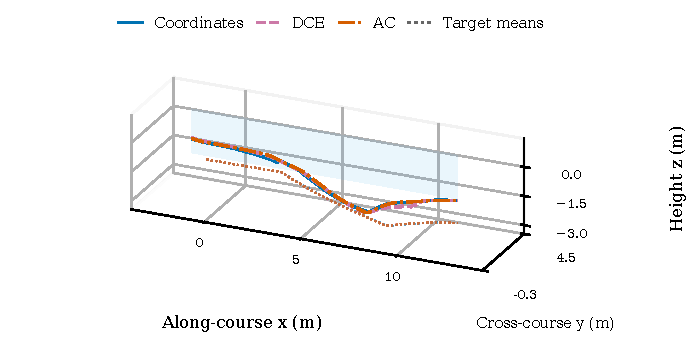
\includegraphics[width=.63\columnwidth]{occlusion_b_mean3d.pdf}\\[-1mm]
{\footnotesize (a) Camera views\hspace{12mm}(b) Mean trajectories}\\[1mm]
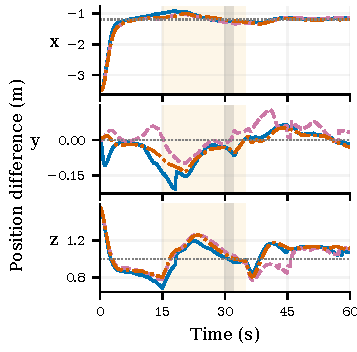
\includegraphics[width=.32\columnwidth]{occlusion_c_relative.pdf}\hfill
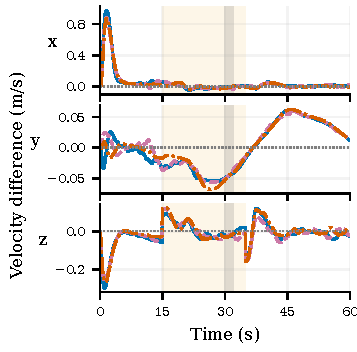
\includegraphics[width=.32\columnwidth]{occlusion_d_velocity.pdf}\hfill
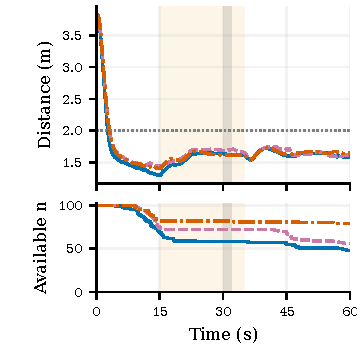
\includegraphics[width=.32\columnwidth]{occlusion_e_distance_count.pdf}\\[-1mm]
{\footnotesize (c) Relative position\hfill(d) Velocity\hfill(e) Range/count}
\caption{Maneuvering pursuit. The target follows a curved path. Gray shading marks the observation gap. Panel definitions follow Fig.~\ref{fig:straight}.}
\label{fig:curved}
\end{inlinefigure}

\newpage
Table~\ref{tab:success} reports complete-mission outcomes. AC achieved the highest observed counts, but three policy seeds do not establish a definitive ranking. It also requires nine predictive rollouts per action. Removing confidence preserves coordinate geometry while eliminating DCE bearing features. Thus intervention sensitivity and ordinary tracking success describe different properties. Figures~\ref{fig:straight}--\ref{fig:curved} retain trajectories, relative motion and surviving-trial counts.

\begin{inlinetable}
\caption{Complete-mission successes out of 100 per cell.}
\label{tab:success}
\footnotesize
\begin{tabular}{@{}llrr@{}}\toprule
Detector & State & Straight & Maneuvering\\\midrule
YOLO26n & Coordinates & 58 & 42\\
YOLO26n & DCE & 54 & 50\\
YOLO26n & AC & 63 & 72\\
ORB & Coordinates / DCE / AC & 0 / 0 / 0 & 0 / 0 / 0\\\bottomrule
\end{tabular}
\end{inlinetable}

The physical recordings in Fig.~\ref{fig:field} document approach and water entry in one lake experiment. Their clocks are unsynchronized. Offline YOLO boxes retain missed detections. These observations are qualitative; synchronized position and control logs are unavailable for scoring the frozen policies in the field.

\begin{inlinefigure}
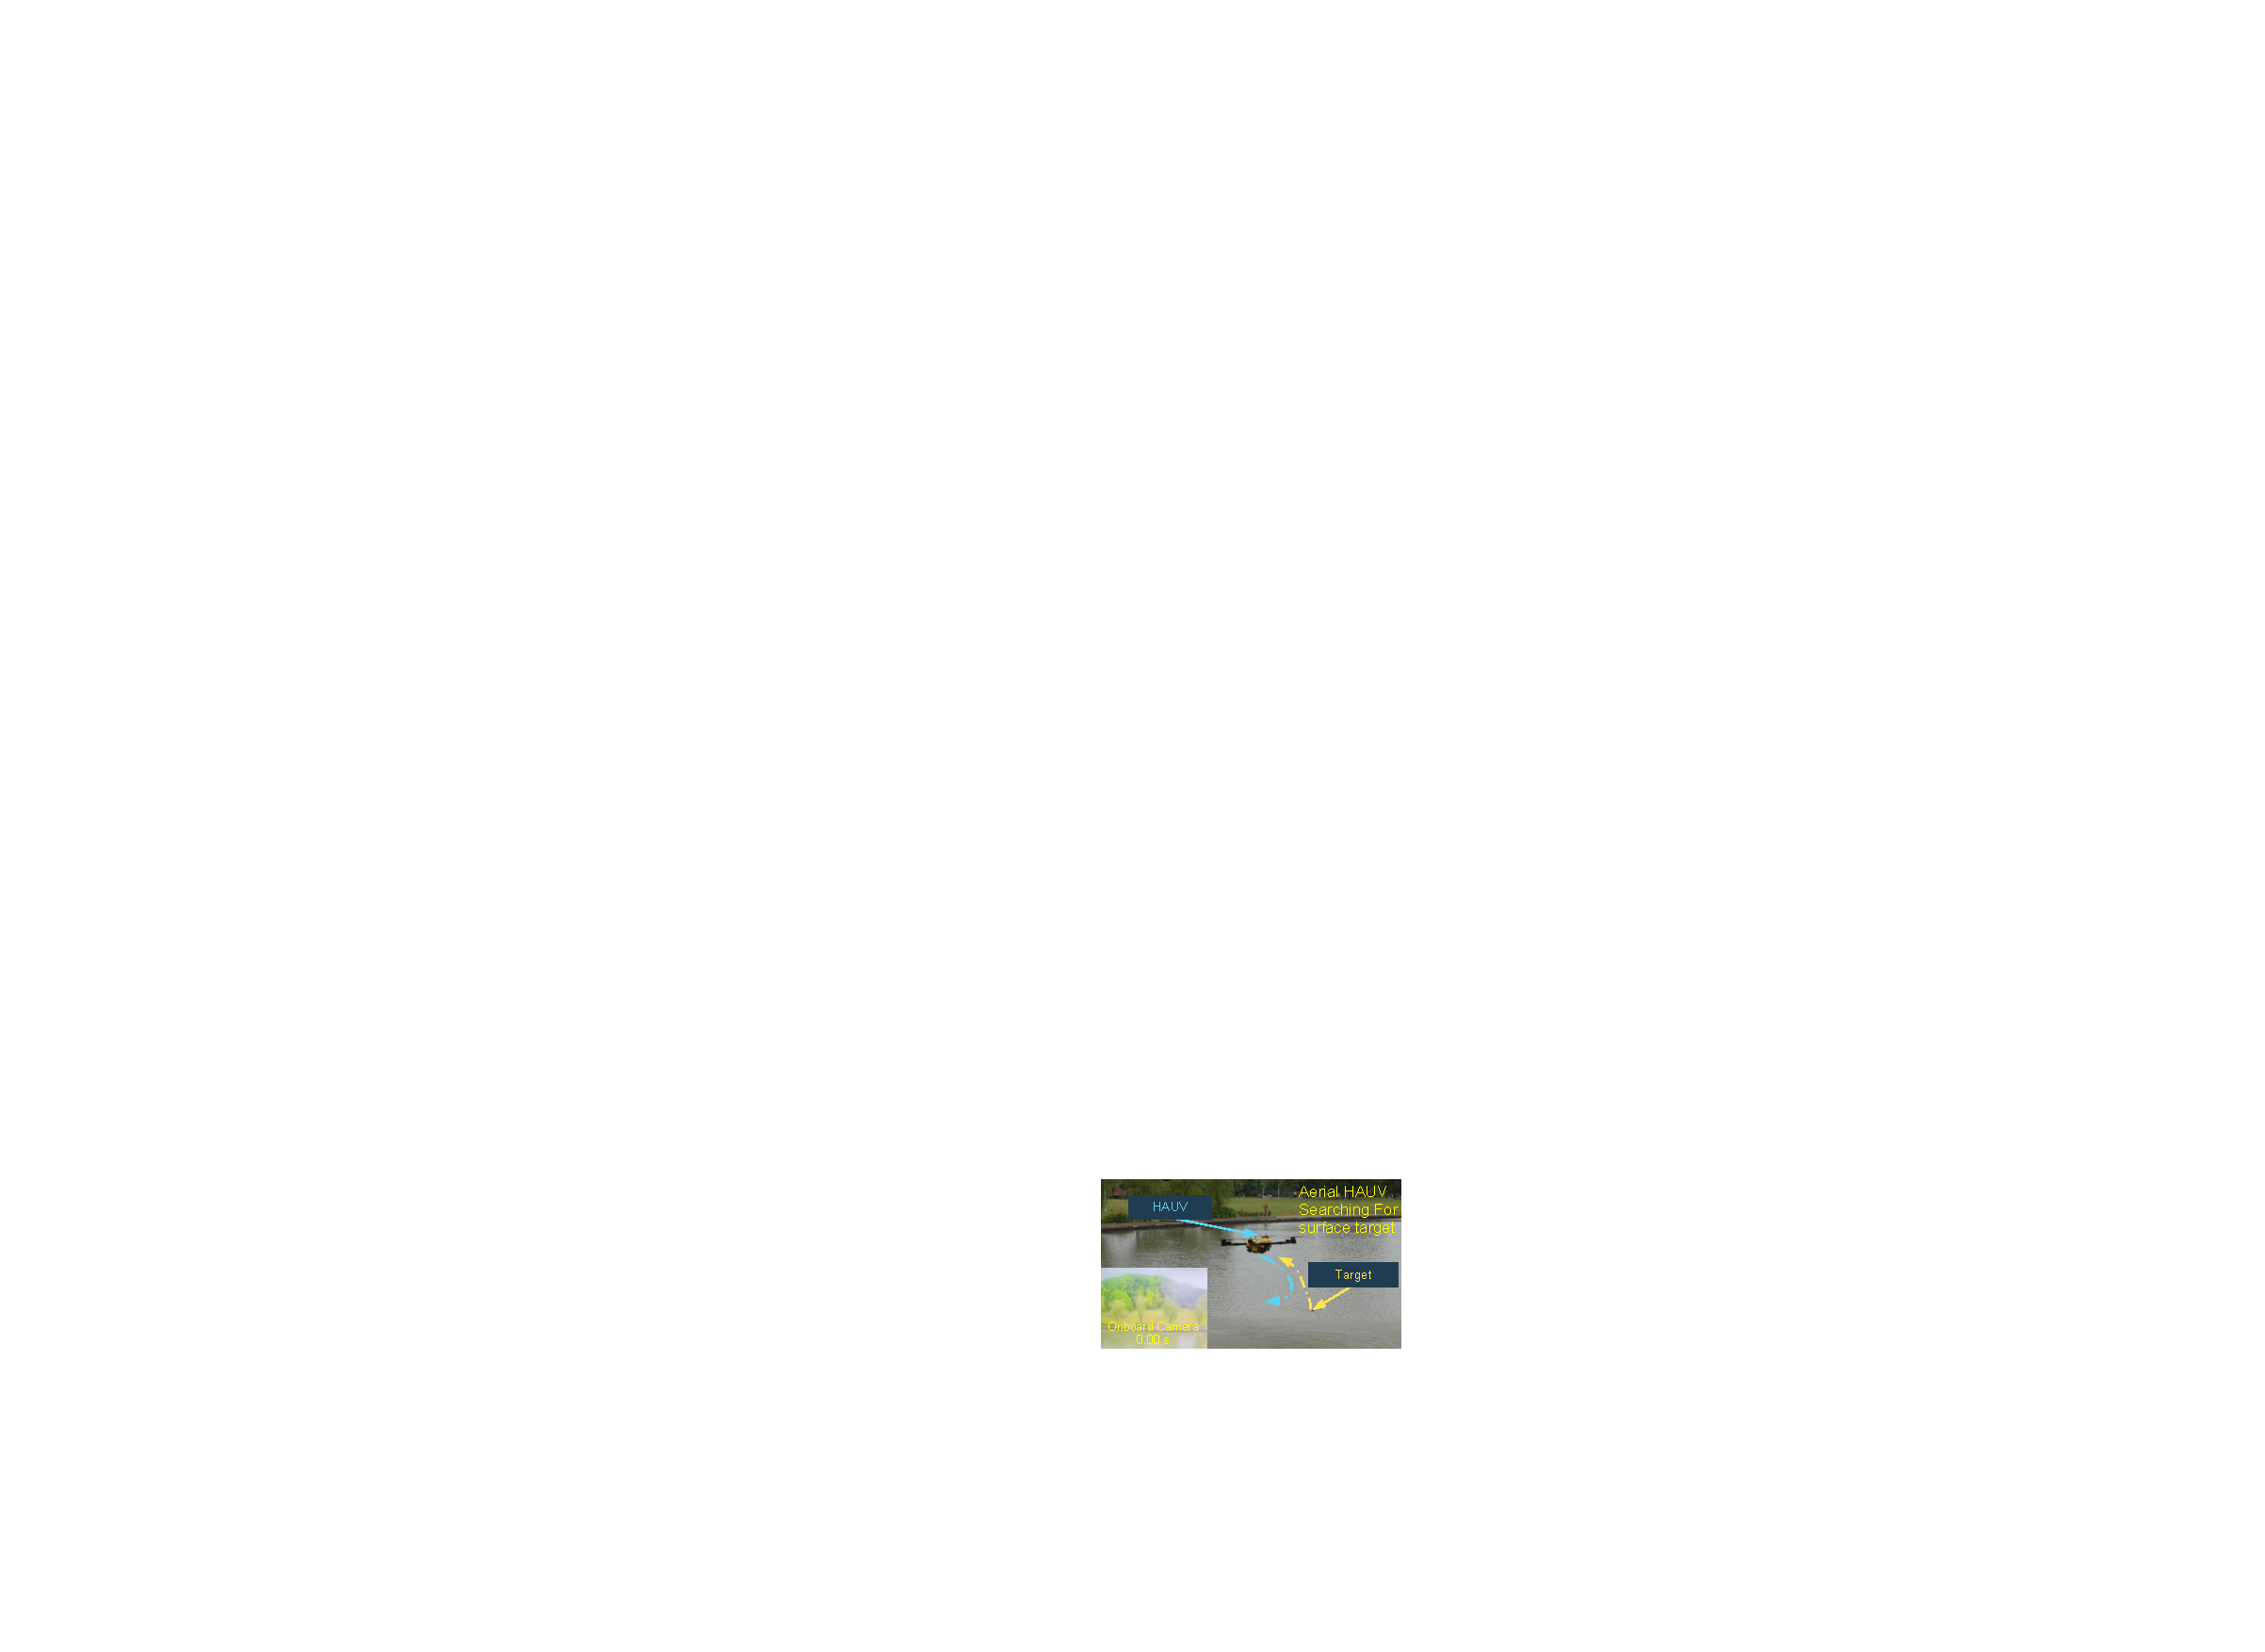
\includegraphics[width=.485\columnwidth]{fig_field1.pdf}\hfill
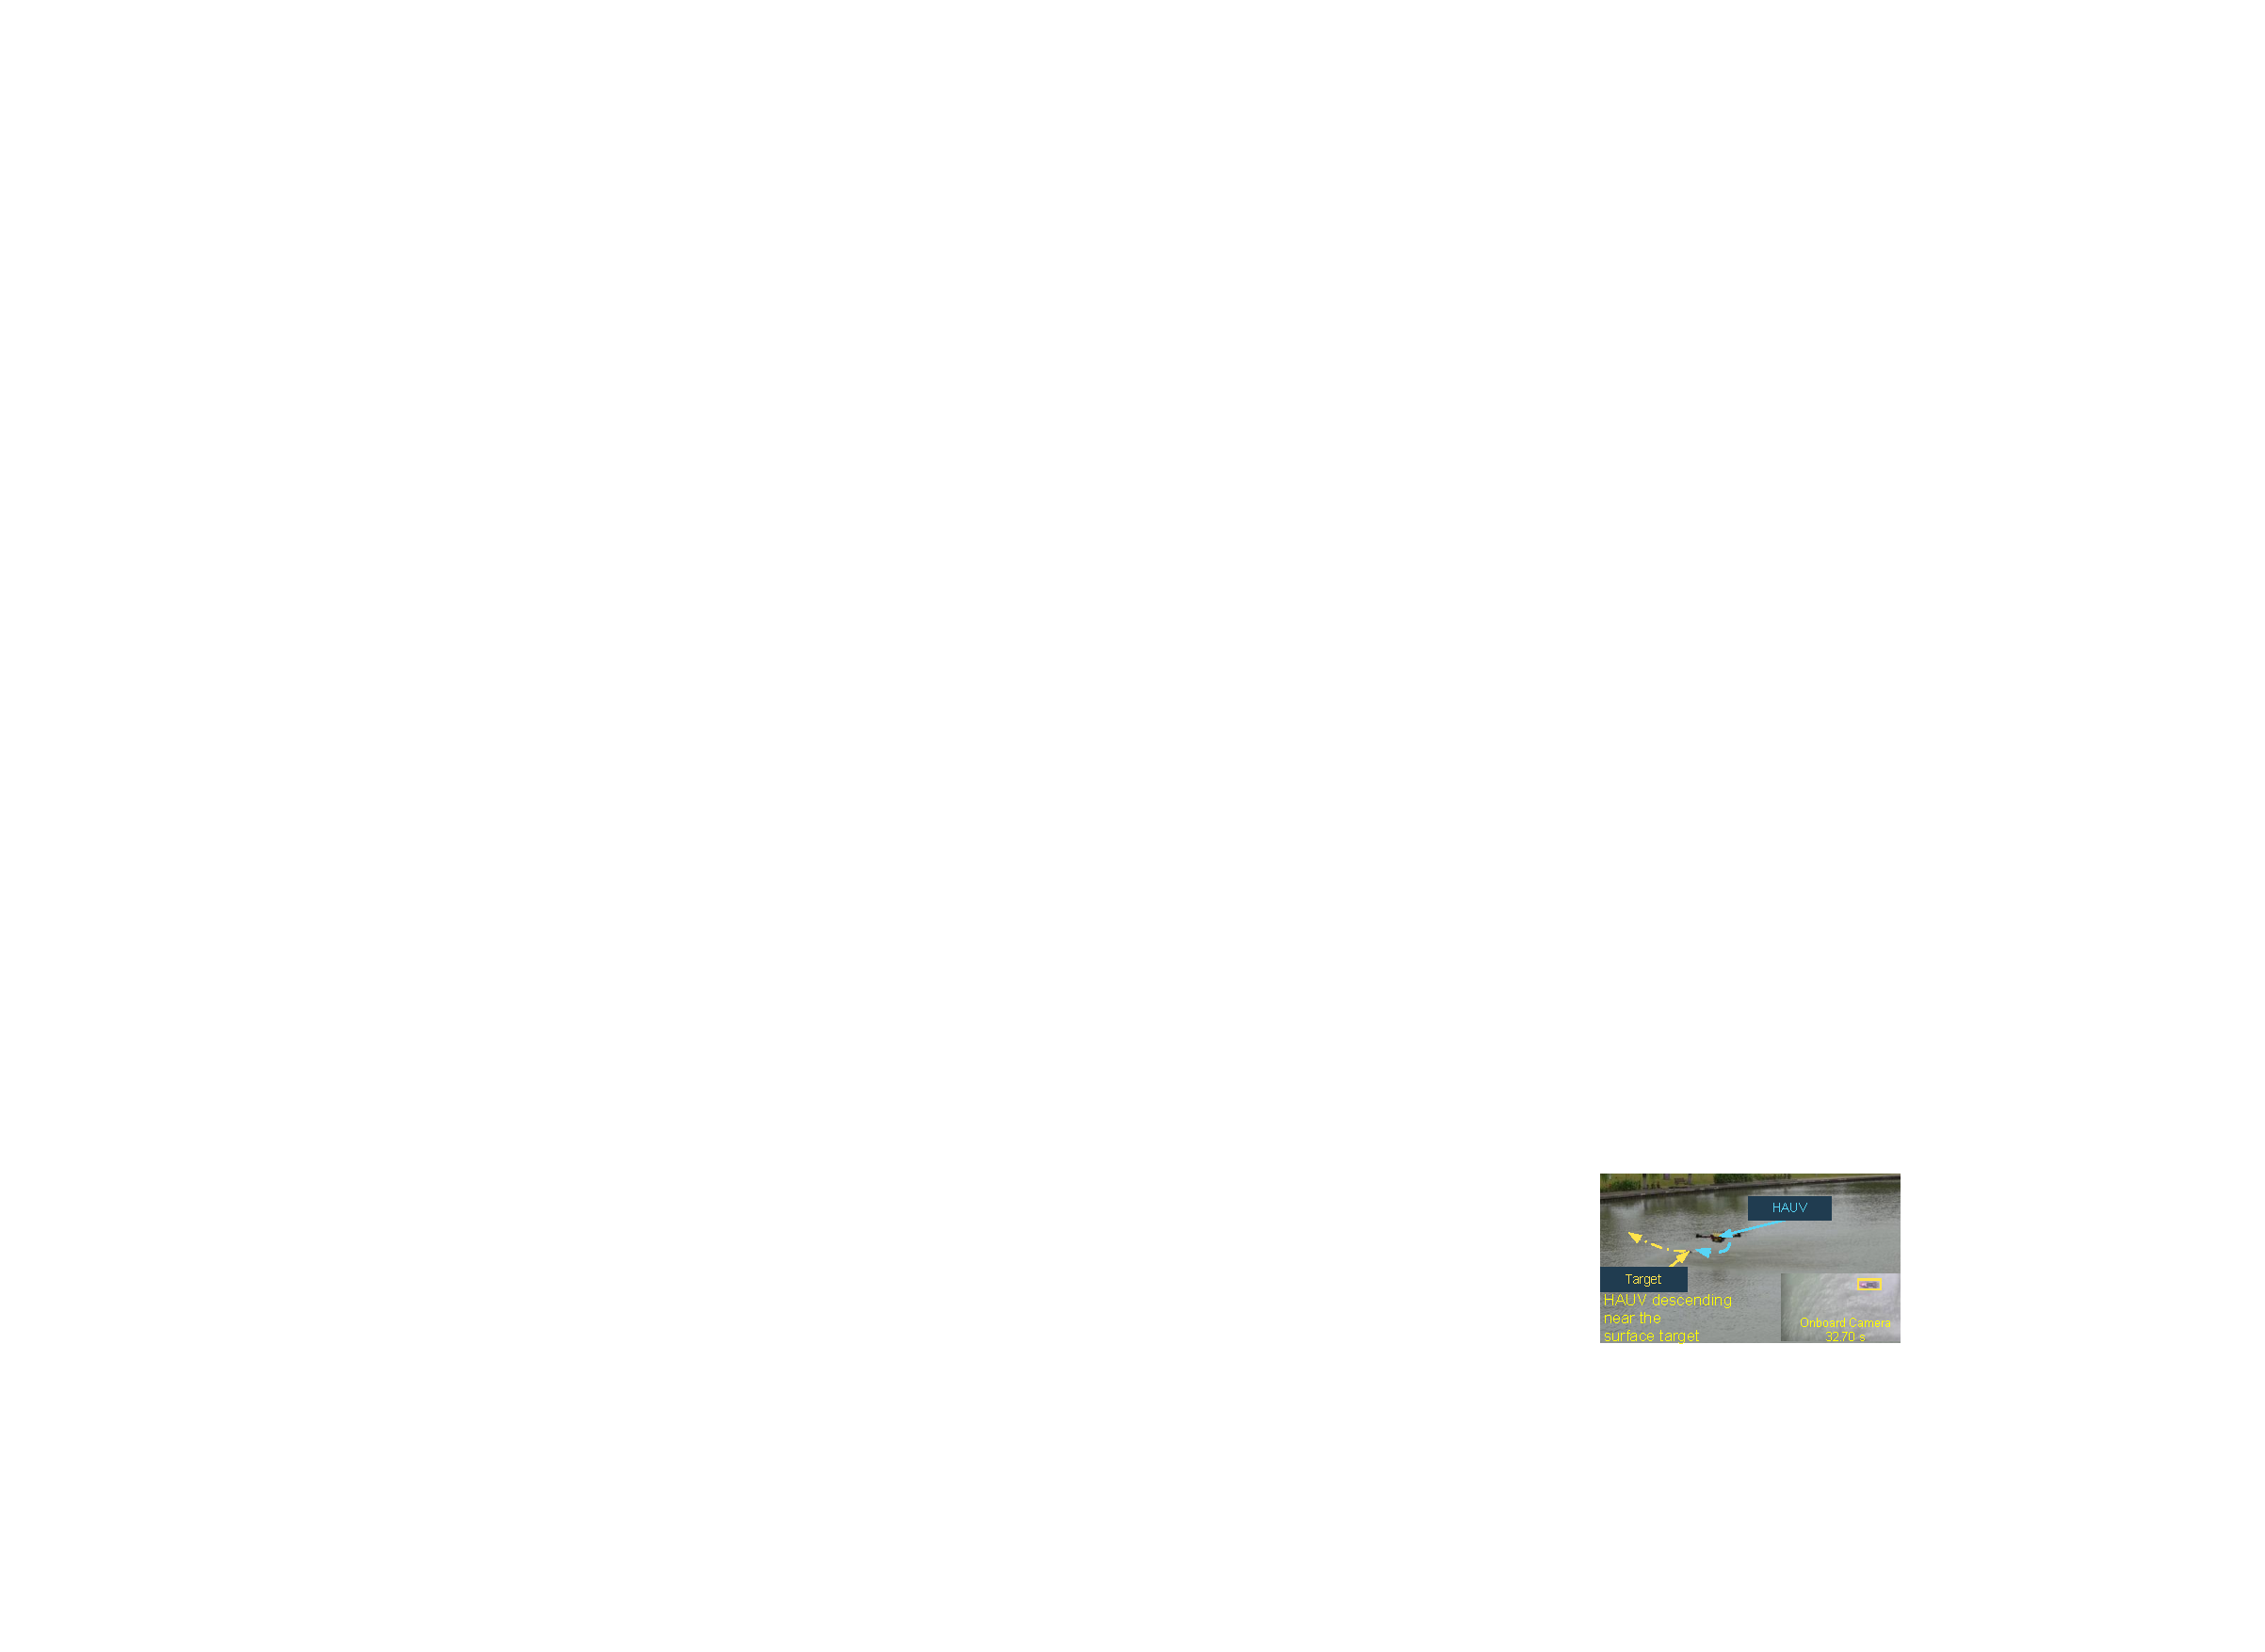
\includegraphics[width=.485\columnwidth]{fig_field2.pdf}\\[1mm]
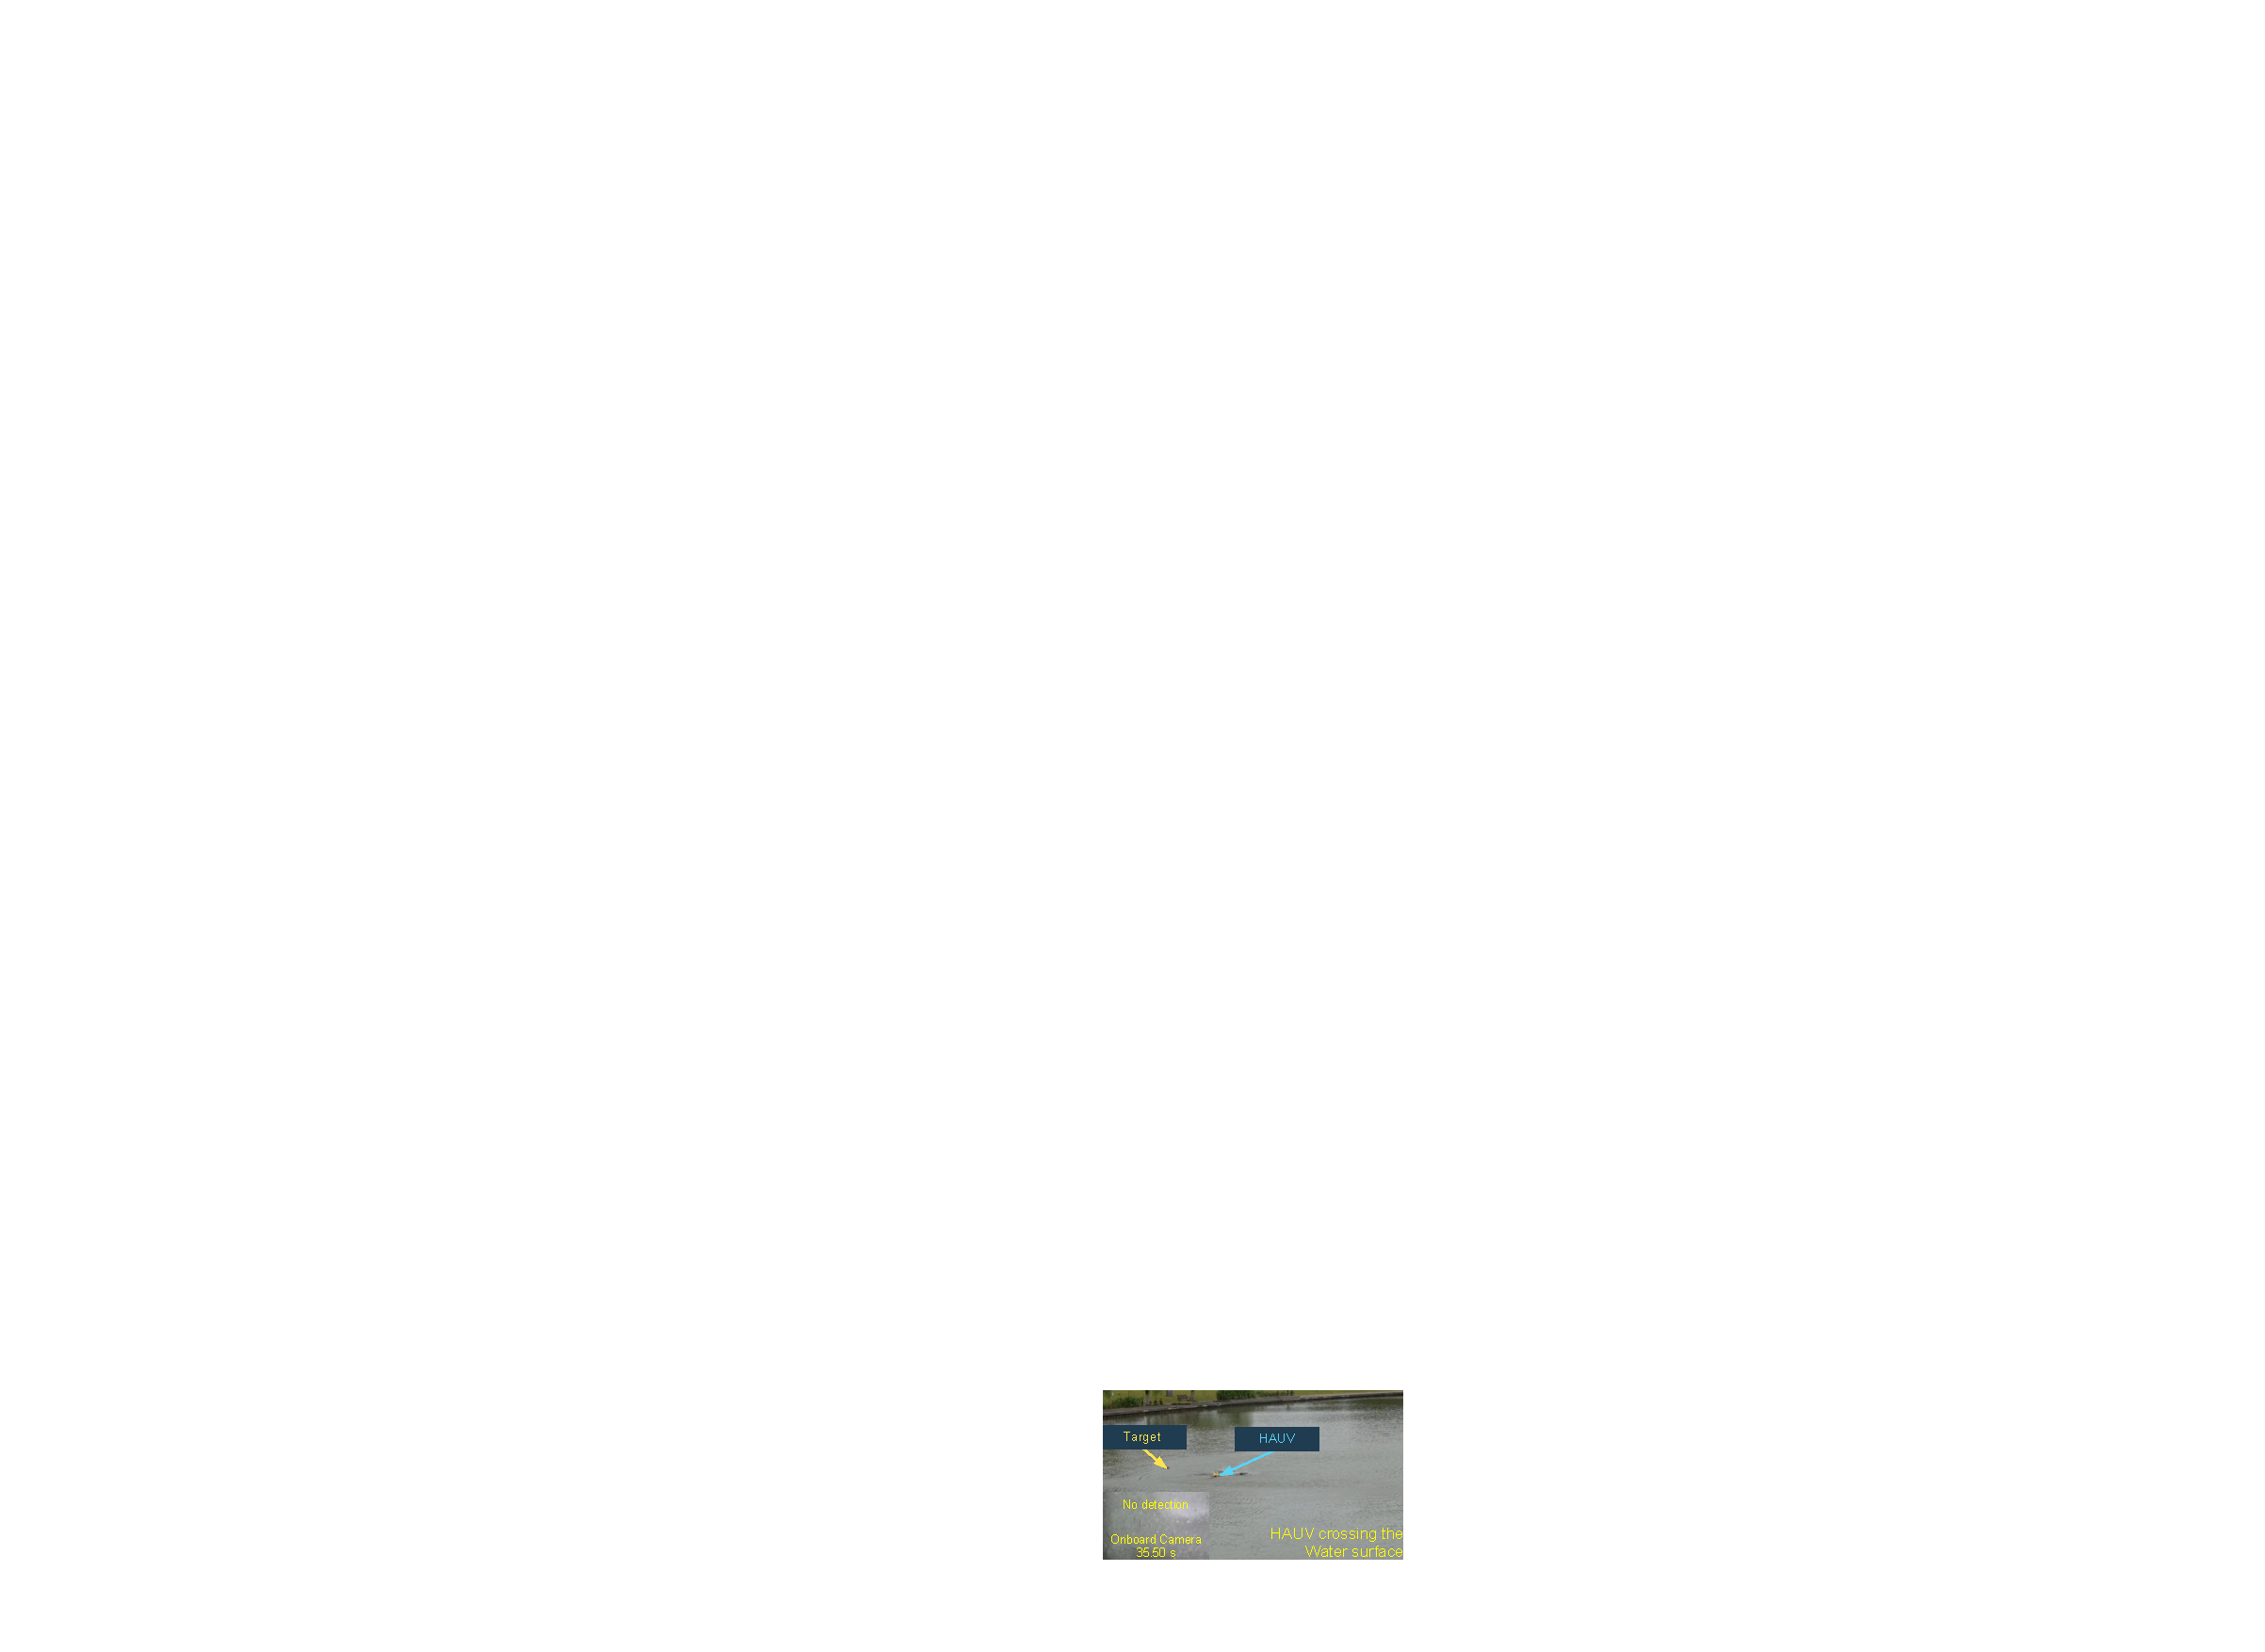
\includegraphics[width=.485\columnwidth]{fig_field3.pdf}\hfill

\includegraphics[width=.485\columnwidth]{fig_field4.pdf}
\caption{Physical approach and water entry. Third-person views and onboard insets retain their separate recording clocks. Detection loss under surface disturbance and underwater turbidity is preserved.}
\label{fig:field}
\end{inlinefigure}

\noindent\textbf{Open materials.} Control weights, loading code and both scenario videos are available at\\
{\footnotesize\url{https://panzerjagerWang.github.io/ut27-hauv-tracking/}}

\begin{thebibliography}{4}
\bibitem{nezha} Y. Bi, Y. Jin, C. Lyu, Z. Zeng and L. Lian, ``Nezha-Mini: Design and locomotion of a miniature low-cost hybrid aerial underwater vehicle,'' \emph{IEEE Robot. Autom. Lett.}, vol. 7, pp. 6669--6676, 2022.
\bibitem{yolo} Ultralytics, ``Ultralytics YOLO26,'' 2026. [Online]. Available: \url{https://docs.ultralytics.com/models/yolo26/}
\bibitem{orb} E. Rublee, V. Rabaud, K. Konolige and G. Bradski, ``ORB: An efficient alternative to SIFT or SURF,'' in \emph{Proc. ICCV}, 2011, pp. 2564--2571.
\bibitem{td3} S. Fujimoto, H. van Hoof and D. Meger, ``Addressing function approximation error in actor-critic methods,'' in \emph{Proc. ICML}, 2018, pp. 1587--1596.
\end{thebibliography}
\end{document}
